% Drawing 154/02-19 -- folder 154, batch 02, archive page 27 (PDF page 28).
% Transcription: figures : deux disques au bord vert, traversés de pseudo-droites orange ; le premier hachuré au crayon sur sa moitié gauche, le second avec des régions triangulaires coloriées en jaune au bord
% Kind: two disks crossed by pseudo-lines. Method 2 (schematic redraw from the facsimile). Status: partial.
% Notes: Each disk: rim dark green on the left half, light green on the right; the orange strands are followed one by one from rim to rim on a gridded crop, ends put on the rim. First disk: two strands share both ends (top and bottom of the rim) and bound a lens, the half of the disk left of it is hatched in pencil; ten strands in all, two of them stopping inside the disk under a pencil scribble, as on the page. Second disk: seven strands, a row of light green dashes along the left of the vertical one, four coloured regions (top, bottom left, right, and a small triangle at the centre). The strands are smooth curves through read points: the order of the crossings along each strand is as read, but near triple points it is not sure. Redrawn 2026-11-12 (issue 128): to check again. 2026-11-14, Claude Opus 5.5, overlay check (issue 147): rasterised from its own coordinates over the 400 dpi colour scan on a unit grid and measured against the colour masks of the ink; not compiled (no TeX in the session); the redraw is unchanged. The strands of both disks lie on their orange ink, except two in the first disk that are 1 to 2 units off over part of their length. Stays partial: the pencil hatching of the left half of the first disk is drawn as a pattern fill, not as the page's long diagonal pencil strokes; the coloured regions of the second disk are drawn as hatched patterns; the order of the crossings near triple points remains a reading.
% Coordinates: 1 unit = 1 mm = 1/100 of the crop width (bbox in page fractions: [0.55, 0.315, 0.87, 0.48]).
% Redrawn by Claude (claude-fable-5-2), issue #128, 2026-11-12; not checked by a human; not compiled (no TeX in the session).
% Checked by Claude (claude-opus-5-5) 2026-11-14 (issue #147): overlaid on the 400 dpi colour facsimile; not compiled (no TeX in the session). Not checked by a human. Status: partial.
% Rights: reproduces part of the work -- behind RENDER_TRANSCRIPTS, never published by itself.
\documentclass[tikz,border=3pt]{standalone}
\usepackage{amsmath,amssymb}
\usetikzlibrary{patterns,arrows.meta}
\tikzset{Or/.style={orange!90!black}, Ye/.style={yellow!80!orange}, Lg/.style={green!60!black!70}, Dg/.style={green!45!black}, pencil/.style={black!45}, struck/.style={black!35}, mpt/.style={circle,draw,inner sep=1.3pt}, pt/.style={circle,fill,inner sep=0.9pt}, opt/.style={circle,draw,fill=white,inner sep=1.1pt}}
\begin{document}
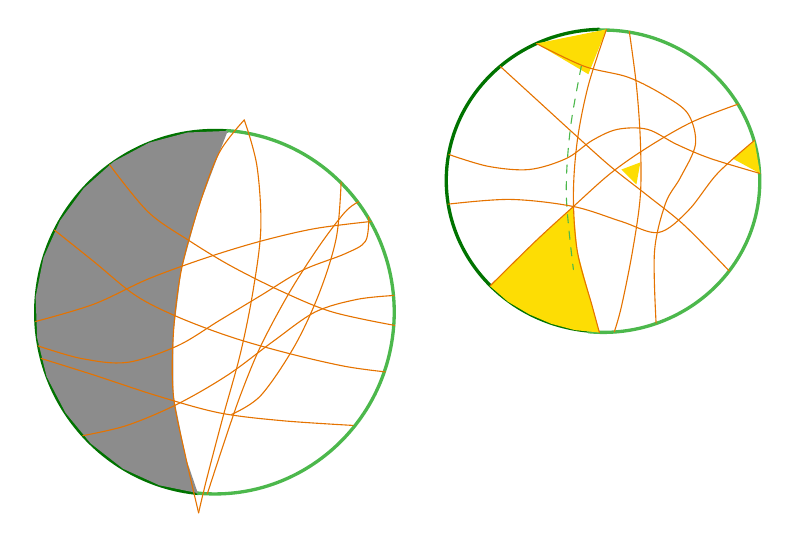
\begin{tikzpicture}[x=1mm,y=1mm,line cap=round,line join=round,font=\scriptsize]
\draw[Dg,very thick] (30.3,-19.9) arc[start angle=86, end angle=264.6, x radius=22.8, y radius=23.1];
\draw[Lg,very thick] (26.5,-65.9) arc[start angle=264.6, end angle=446, x radius=22.8, y radius=23.1];
\fill[pattern=north east lines,pencil] (30.3,-19.9) -- (25.2,-20.1) -- (20.3,-21.4) -- (15.8,-23.8) -- (12,-27.2) -- (9,-31.3) -- (6.9,-36) -- (5.9,-41) -- (6.1,-46.2) -- (7.3,-51.1) -- (9.7,-55.7) -- (12.9,-59.6) -- (17,-62.8) -- (21.6,-64.9) -- (26.5,-65.9) -- (25,-61.5) -- (23.4,-53.5) -- (23.4,-45.6) -- (24.4,-37.6) -- (26.6,-29.6) -- (29.2,-22.7) -- cycle;
\draw[Or] plot[smooth, tension=0.55] coordinates {(32.4,-18.5) (34,-24.3) (34.5,-32.3) (33.5,-40.3) (31.9,-48.2) (29.7,-56.2) (27.6,-64.2) (26.6,-68.4)};
\draw[Or] plot[smooth, tension=0.55] coordinates {(32.4,-18.5) (29.2,-22.7) (26.6,-29.6) (24.4,-37.6) (23.4,-45.6) (23.4,-53.5) (25,-61.5) (26.6,-68.4)};
\draw[Or] plot[smooth, tension=0.55] coordinates {(15.3,-24.2) (20.2,-30.2) (25.5,-33.9) (30.8,-37.1) (37.2,-40.3) (43.6,-42.9) (51.5,-44.6)};
\draw[Or] plot[smooth, tension=0.55] coordinates {(8.3,-32.5) (13.3,-36.5) (18.6,-40.8) (23.9,-43.5) (30.8,-46.1) (38.2,-48.2) (45.2,-49.8) (50.3,-50.5)};
\draw[Or] plot[smooth, tension=0.55] coordinates {(5.9,-44.1) (13.3,-41.9) (20.2,-38.7) (27.6,-36) (34.5,-33.9) (41.4,-32.3) (48.5,-31.4)};
\draw[Or] plot[smooth, tension=0.55] coordinates {(6.2,-47.2) (11.7,-48.8) (17.5,-49.3) (23.9,-47.2) (29.2,-44) (34.5,-40.8) (39.8,-37.6) (45.2,-35.5) (47.8,-33.9) (48.2,-30.8)};
\draw[Or] plot[smooth, tension=0.55] coordinates {(6.6,-48.8) (13.3,-50.9) (21.2,-53.5) (29.2,-55.7) (37.2,-56.7) (46.2,-57.3)};
\draw[Or] plot[smooth, tension=0.55] coordinates {(11.9,-58.6) (17.5,-57.3) (23.9,-54.6) (30.3,-50.9) (36.1,-46.6) (41.4,-42.9) (46.7,-41.3) (51.4,-40.8)};
\draw[Or] plot[smooth, tension=0.55] coordinates {(27.7,-66) (29.7,-59.9) (31.9,-53.5) (34.5,-47.2) (38.2,-40.3) (42,-34.4) (45.2,-30.2) (46.9,-28.9)};
\draw[Or] plot[smooth, tension=0.55] coordinates {(44.7,-26.4) (44.1,-33.4) (42,-40.3) (38.8,-47.2) (34.5,-53.5) (30.8,-55.9)};
\draw[Dg,very thick] (77.5,-7) arc[start angle=91.3, end angle=264.6, x radius=19.9, y radius=19.2];
\draw[Lg,very thick] (76.1,-45.4) arc[start angle=264.6, end angle=451.3, x radius=19.9, y radius=19.2];
\fill[pattern=north east lines,Ye] (69.5,-8.8) -- (78.4,-7) -- (76.1,-12.7) -- cycle;
\fill[pattern=north east lines,Ye] (63.6,-39.6) -- (69.5,-33.8) -- (74.2,-29.5) -- (74.7,-35.2) -- (76.6,-42.2) -- (77.5,-45.5) -- (74.4,-45.2) -- (71.4,-44.4) -- (68.6,-43.2) -- (65.9,-41.6) -- (63.6,-39.6) -- cycle;
\fill[pattern=north east lines,Ye] (94.4,-23.4) -- (97.2,-21.2) -- (97.9,-25.3) -- cycle;
\fill[pattern=north east lines,Ye] (80.3,-24.8) -- (82.7,-23.9) -- (82.2,-26.7) -- cycle;
\draw[Or] plot[smooth, tension=0.55] coordinates {(78.4,-7) (76.1,-14.1) (74.7,-21.1) (74.2,-28.1) (74.7,-35.2) (76.6,-42.2) (77.5,-45.5)};
\draw[Lg,dashed] plot[smooth, tension=0.55] coordinates {(75.2,-11.7) (73.8,-19.7) (73.3,-28.1) (74.2,-37.5)};
\draw[Or] plot[smooth, tension=0.55] coordinates {(64.9,-11.7) (69.5,-15.9) (74.2,-20.2) (78.9,-24.4) (83.6,-28.1) (88.3,-31.9) (94,-37.7)};
\draw[Or] plot[smooth, tension=0.55] coordinates {(69.5,-8.8) (75.6,-11.7) (81.2,-13.1) (85.9,-15.5) (88.8,-17.8) (89.7,-21.6) (87.8,-25.8) (85.9,-29.1) (84.5,-35.2) (84.7,-44.3)};
\draw[Or] plot[smooth, tension=0.55] coordinates {(81.3,-7.3) (82.2,-14.1) (82.7,-21.1) (82.7,-28.1) (81.7,-35.2) (80.3,-42.2) (79.4,-45.4)};
\draw[Or] plot[smooth, tension=0.55] coordinates {(58.4,-22.9) (63.4,-24.4) (68.6,-24.8) (73.3,-23.4) (76.6,-21.1) (79.8,-19.7) (83.6,-19.7) (87.3,-21.6) (91.6,-23.4) (97.9,-25.3)};
\draw[Or] plot[smooth, tension=0.55] coordinates {(58.3,-29.2) (66.2,-28.6) (74.2,-29.5) (80.3,-31.4) (85,-32.8) (88.8,-30) (92.5,-25.3) (97.2,-21.1)};
\draw[Or] plot[smooth, tension=0.55] coordinates {(63.6,-39.6) (69.5,-33.8) (74.2,-29.5) (78.9,-25.3) (83.6,-22) (89.2,-18.8) (95.1,-16.5)};
\end{tikzpicture}
\end{document}
